% Section: Multi-Model Evaluation — K=5 and K=10
% Include from the main paper via % Section: Multi-Model Evaluation — K=5 and K=10
% Include from the main paper via % Section: Multi-Model Evaluation — K=5 and K=10
% Include from the main paper via % Section: Multi-Model Evaluation — K=5 and K=10
% Include from the main paper via \input{../experiments/06_figure/section_multimodel_results}

\subsection{Multi-Model Cost--Quality Trade-off ($K{=}5, 10$)}
\label{sec:multimodel}

We construct two multi-provider portfolios ($K{=}5$ and $K{=}10$) spanning six providers (Meta, Mistral, Google, Anthropic, OpenAI, DeepSeek) with a $600\times$ cost spread. Both incorporate Mixtral-8x7B to link to the $K{=}2$ evaluation, and $K{=}10$ exercises Hybrid LinUCB's within-family parameter sharing. Warmup priors are generated using a three-way split from 43-model evaluation data (355 prior training prompts, 533 online learning, 750 holdout).

\input{../experiments/06_figure/figure_6_caption}

\paragraph{Continuous cost--quality control.}
Table~\ref{tab:multimodel_summary} and Figure~\ref{fig:multimodel_pareto} summarize the findings. By sweeping a single scalar ($\lambda$), the router traces a smooth operating envelope. At $K{=}10$, quality degrades only 1\% ($0.898 \to 0.888$) across a $41\times$ cost range because the portfolio contains cheap, high-quality models (Gemma-3-27B, DeepSeek-V3) that the router leverages at higher $\lambda$ values.

\begin{table}[h]
\centering
\caption{Multi-model routing summary (mean judge agreement). Gap closure is relative to the weakest model. Mean $\pm$ std ($n{=}20$).}
\label{tab:multimodel_summary}
\small
\resizebox{\columnwidth}{!}{%
\begin{tabular}{@{}lcc@{}}
\toprule
\textbf{Metric} & \textbf{K=5} & \textbf{K=10} \\
\midrule
Oracle                     & 0.986              & 0.991 \\
Best Static (GPT-4.1)      & 0.949              & 0.949 \\
Random                     & 0.844 $\pm$ 0.008  & 0.857 $\pm$ 0.007 \\
\midrule
banditGPT Peak Quality     & 0.911 $\pm$ 0.022  & 0.898 $\pm$ 0.023 \\
Gap Closure                & 74.9\%              & 69.3\% \\
Warmup Cold-Start (step 0) & 0.898 $\pm$ 0.007  & 0.903 $\pm$ 0.006 \\
\midrule
Cost vs.\ Best Static at $\lambda{=}0$ & 9\% cheaper         & 36\% cheaper \\
Cost vs.\ Best Static at $\lambda{=}5$ & 98.7\% cheaper      & 98.4\% cheaper \\
\bottomrule
\end{tabular}%
}
\end{table}

\paragraph{Zero cold-start and distributed traffic.}
At step~0 (before online learning), banditGPT achieves holdout quality within 9\% of the Oracle. Online, traffic distributes across the portfolio based on prompt context. At $K{=}5$, three strong models share ${\sim}90\%$ of traffic; at $K{=}10$, no model exceeds 17\% (Figure~\ref{fig:multimodel_pareto}d). This provides immense operational resilience: a single-provider outage limits impact to a fraction of traffic, which the router autonomously redistributes.

\paragraph{Exploration-exploitation overhead.}
At peak $\lambda$, banditGPT's quality is slightly below the best static model (GPT-4.1). This reflects the bandit's structural exploration cost (testing sub-optimal models to verify calibration), which grows with $K$. However, this exploration enables a $91\%$ cost reduction at $\lambda{=}1.0$ relative to static GPT-4.1 with only a 6.1\% quality drop, a trade-off inaccessible to static baselines.

\paragraph{Static Pareto frontier and per-prompt value.}
The static Pareto frontier in Figure~\ref{fig:multimodel_pareto}(a,b) reveals which models are non-dominated when routing all traffic to a single endpoint. At $K{=}5$, only three of five models are Pareto-efficient (Llama-3.1-8B, Gemini-2.5-Flash, GPT-4.1); Mixtral-8x7B is dominated by Gemini-Flash (cheaper \emph{and} higher quality), and Claude-Sonnet-4 is dominated by GPT-4.1. Yet banditGPT routes 32\% of $K{=}5$ traffic to Claude-Sonnet-4 (Figure~\ref{fig:multimodel_pareto}d), indicating it provides unique value on specific prompt subsets despite being dominated in aggregate. This disconnect between aggregate dominance and per-prompt utility is precisely the Quality Inversion phenomenon that contextual routing exploits: a model that is strictly inferior on average can still be the best choice for a measurable fraction of prompts.


\subsection{Multi-Model Cost--Quality Trade-off ($K{=}5, 10$)}
\label{sec:multimodel}

We construct two multi-provider portfolios ($K{=}5$ and $K{=}10$) spanning six providers (Meta, Mistral, Google, Anthropic, OpenAI, DeepSeek) with a $600\times$ cost spread. Both incorporate Mixtral-8x7B to link to the $K{=}2$ evaluation, and $K{=}10$ exercises Hybrid LinUCB's within-family parameter sharing. Warmup priors are generated using a three-way split from 43-model evaluation data (355 prior training prompts, 533 online learning, 750 holdout).

% Figure 6: Multi-Model Pareto Frontier — K=5 and K=10
% Include from the main paper via \input{../experiments/06_figure/figure_6_caption}

\begin{figure*}[t]
\centering
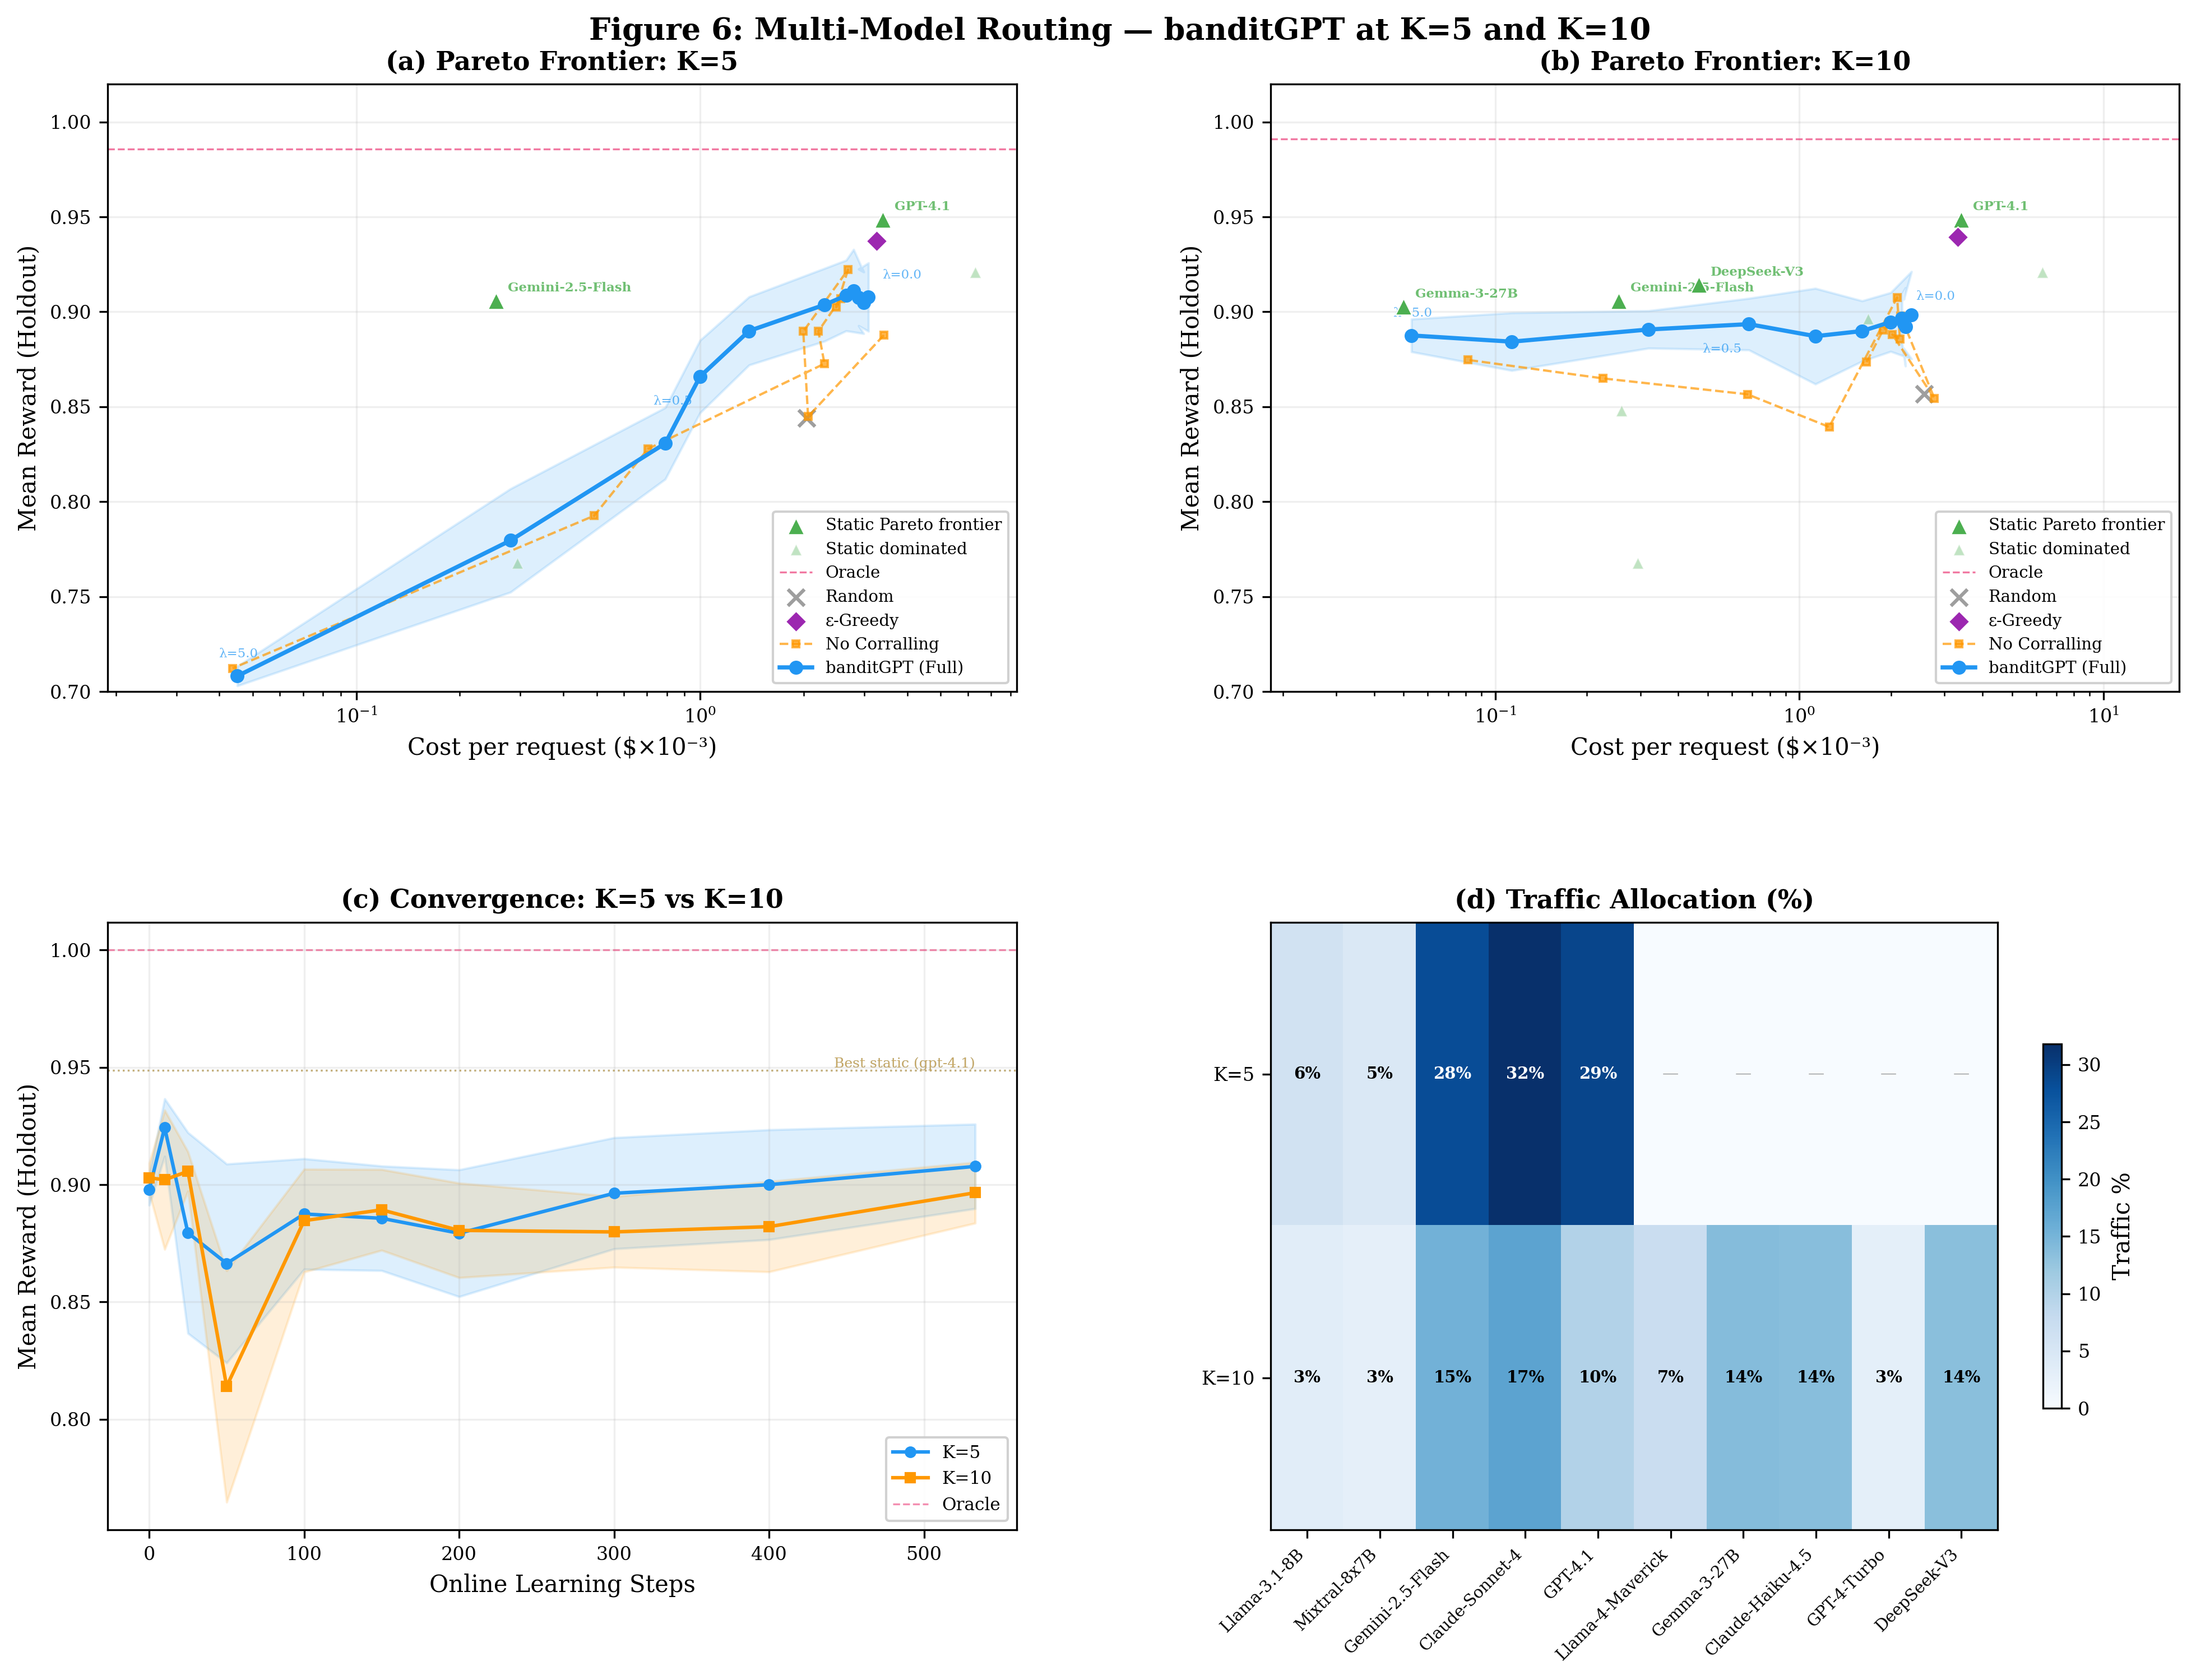
\includegraphics[width=0.95\textwidth]{../experiments/06_figure/results/figure6_multimodel_pareto.png}
\caption{\textbf{Multi-model routing at $K{=}5$ and $K{=}10$: cost--quality Pareto frontiers, convergence, and traffic allocation.} Reward is mean judge agreement across a 3--4 member LLM panel (continuous in $[0,1]$).
\textbf{(a,b)}~Pareto frontiers sweeping cost penalty $\lambda \in [0, 5]$ ($n{=}20$ seeds per point; log-scaled cost axis). Labelled green triangles mark Pareto-efficient static baselines; faded triangles show dominated models. The blue curve traces banditGPT's operating envelope. At peak quality ($\lambda{=}0.02$), banditGPT achieves 0.911 (K{=}5) and 0.898 (K{=}10). At $\lambda{=}5$ (cost-minimising), it routes nearly all traffic to the cheapest model while maintaining 0.708 (K{=}5) and 0.888 (K{=}10) quality. The orange dashed line (no Corralling) shows the ablated system without the meta-learner.
\textbf{(c)}~Convergence from warmup priors: both portfolios start at ${\sim}0.90$ reward (step~0, no online learning), demonstrating that the 43-model warmup priors provide effective cold-start quality across portfolio sizes. K{=}5 improves to 0.911 by step 533; K{=}10 remains stable at ${\sim}0.88{-}0.90$.
\textbf{(d)}~Traffic allocation on the holdout set ($\lambda{=}0$). At K{=}5, the router concentrates on three high-quality models (Claude-Sonnet: 32\%, GPT-4.1: 29\%, Gemini-Flash: 28\%) while using cheaper models sparingly (${\leq}6\%$). At K{=}10, traffic distributes across all models (3--17\% each), reflecting contextual per-prompt routing rather than static model selection.
Evaluation protocol: 533 online-learning prompts (three-way split, disjoint from prior training), frozen holdout of 750 prompts (identical to Section~\ref{sec:pareto}).}
\label{fig:multimodel_pareto}
\end{figure*}


\paragraph{Continuous cost--quality control.}
Table~\ref{tab:multimodel_summary} and Figure~\ref{fig:multimodel_pareto} summarize the findings. By sweeping a single scalar ($\lambda$), the router traces a smooth operating envelope. At $K{=}10$, quality degrades only 1\% ($0.898 \to 0.888$) across a $41\times$ cost range because the portfolio contains cheap, high-quality models (Gemma-3-27B, DeepSeek-V3) that the router leverages at higher $\lambda$ values.

\begin{table}[h]
\centering
\caption{Multi-model routing summary (mean judge agreement). Gap closure is relative to the weakest model. Mean $\pm$ std ($n{=}20$).}
\label{tab:multimodel_summary}
\small
\resizebox{\columnwidth}{!}{%
\begin{tabular}{@{}lcc@{}}
\toprule
\textbf{Metric} & \textbf{K=5} & \textbf{K=10} \\
\midrule
Oracle                     & 0.986              & 0.991 \\
Best Static (GPT-4.1)      & 0.949              & 0.949 \\
Random                     & 0.844 $\pm$ 0.008  & 0.857 $\pm$ 0.007 \\
\midrule
banditGPT Peak Quality     & 0.911 $\pm$ 0.022  & 0.898 $\pm$ 0.023 \\
Gap Closure                & 74.9\%              & 69.3\% \\
Warmup Cold-Start (step 0) & 0.898 $\pm$ 0.007  & 0.903 $\pm$ 0.006 \\
\midrule
Cost vs.\ Best Static at $\lambda{=}0$ & 9\% cheaper         & 36\% cheaper \\
Cost vs.\ Best Static at $\lambda{=}5$ & 98.7\% cheaper      & 98.4\% cheaper \\
\bottomrule
\end{tabular}%
}
\end{table}

\paragraph{Zero cold-start and distributed traffic.}
At step~0 (before online learning), banditGPT achieves holdout quality within 9\% of the Oracle. Online, traffic distributes across the portfolio based on prompt context. At $K{=}5$, three strong models share ${\sim}90\%$ of traffic; at $K{=}10$, no model exceeds 17\% (Figure~\ref{fig:multimodel_pareto}d). This provides immense operational resilience: a single-provider outage limits impact to a fraction of traffic, which the router autonomously redistributes.

\paragraph{Exploration-exploitation overhead.}
At peak $\lambda$, banditGPT's quality is slightly below the best static model (GPT-4.1). This reflects the bandit's structural exploration cost (testing sub-optimal models to verify calibration), which grows with $K$. However, this exploration enables a $91\%$ cost reduction at $\lambda{=}1.0$ relative to static GPT-4.1 with only a 6.1\% quality drop, a trade-off inaccessible to static baselines.

\paragraph{Static Pareto frontier and per-prompt value.}
The static Pareto frontier in Figure~\ref{fig:multimodel_pareto}(a,b) reveals which models are non-dominated when routing all traffic to a single endpoint. At $K{=}5$, only three of five models are Pareto-efficient (Llama-3.1-8B, Gemini-2.5-Flash, GPT-4.1); Mixtral-8x7B is dominated by Gemini-Flash (cheaper \emph{and} higher quality), and Claude-Sonnet-4 is dominated by GPT-4.1. Yet banditGPT routes 32\% of $K{=}5$ traffic to Claude-Sonnet-4 (Figure~\ref{fig:multimodel_pareto}d), indicating it provides unique value on specific prompt subsets despite being dominated in aggregate. This disconnect between aggregate dominance and per-prompt utility is precisely the Quality Inversion phenomenon that contextual routing exploits: a model that is strictly inferior on average can still be the best choice for a measurable fraction of prompts.


\subsection{Multi-Model Cost--Quality Trade-off ($K{=}5, 10$)}
\label{sec:multimodel}

We construct two multi-provider portfolios ($K{=}5$ and $K{=}10$) spanning six providers (Meta, Mistral, Google, Anthropic, OpenAI, DeepSeek) with a $600\times$ cost spread. Both incorporate Mixtral-8x7B to link to the $K{=}2$ evaluation, and $K{=}10$ exercises Hybrid LinUCB's within-family parameter sharing. Warmup priors are generated using a three-way split from 43-model evaluation data (355 prior training prompts, 533 online learning, 750 holdout).

% Figure 6: Multi-Model Pareto Frontier — K=5 and K=10
% Include from the main paper via % Figure 6: Multi-Model Pareto Frontier — K=5 and K=10
% Include from the main paper via \input{../experiments/06_figure/figure_6_caption}

\begin{figure*}[t]
\centering
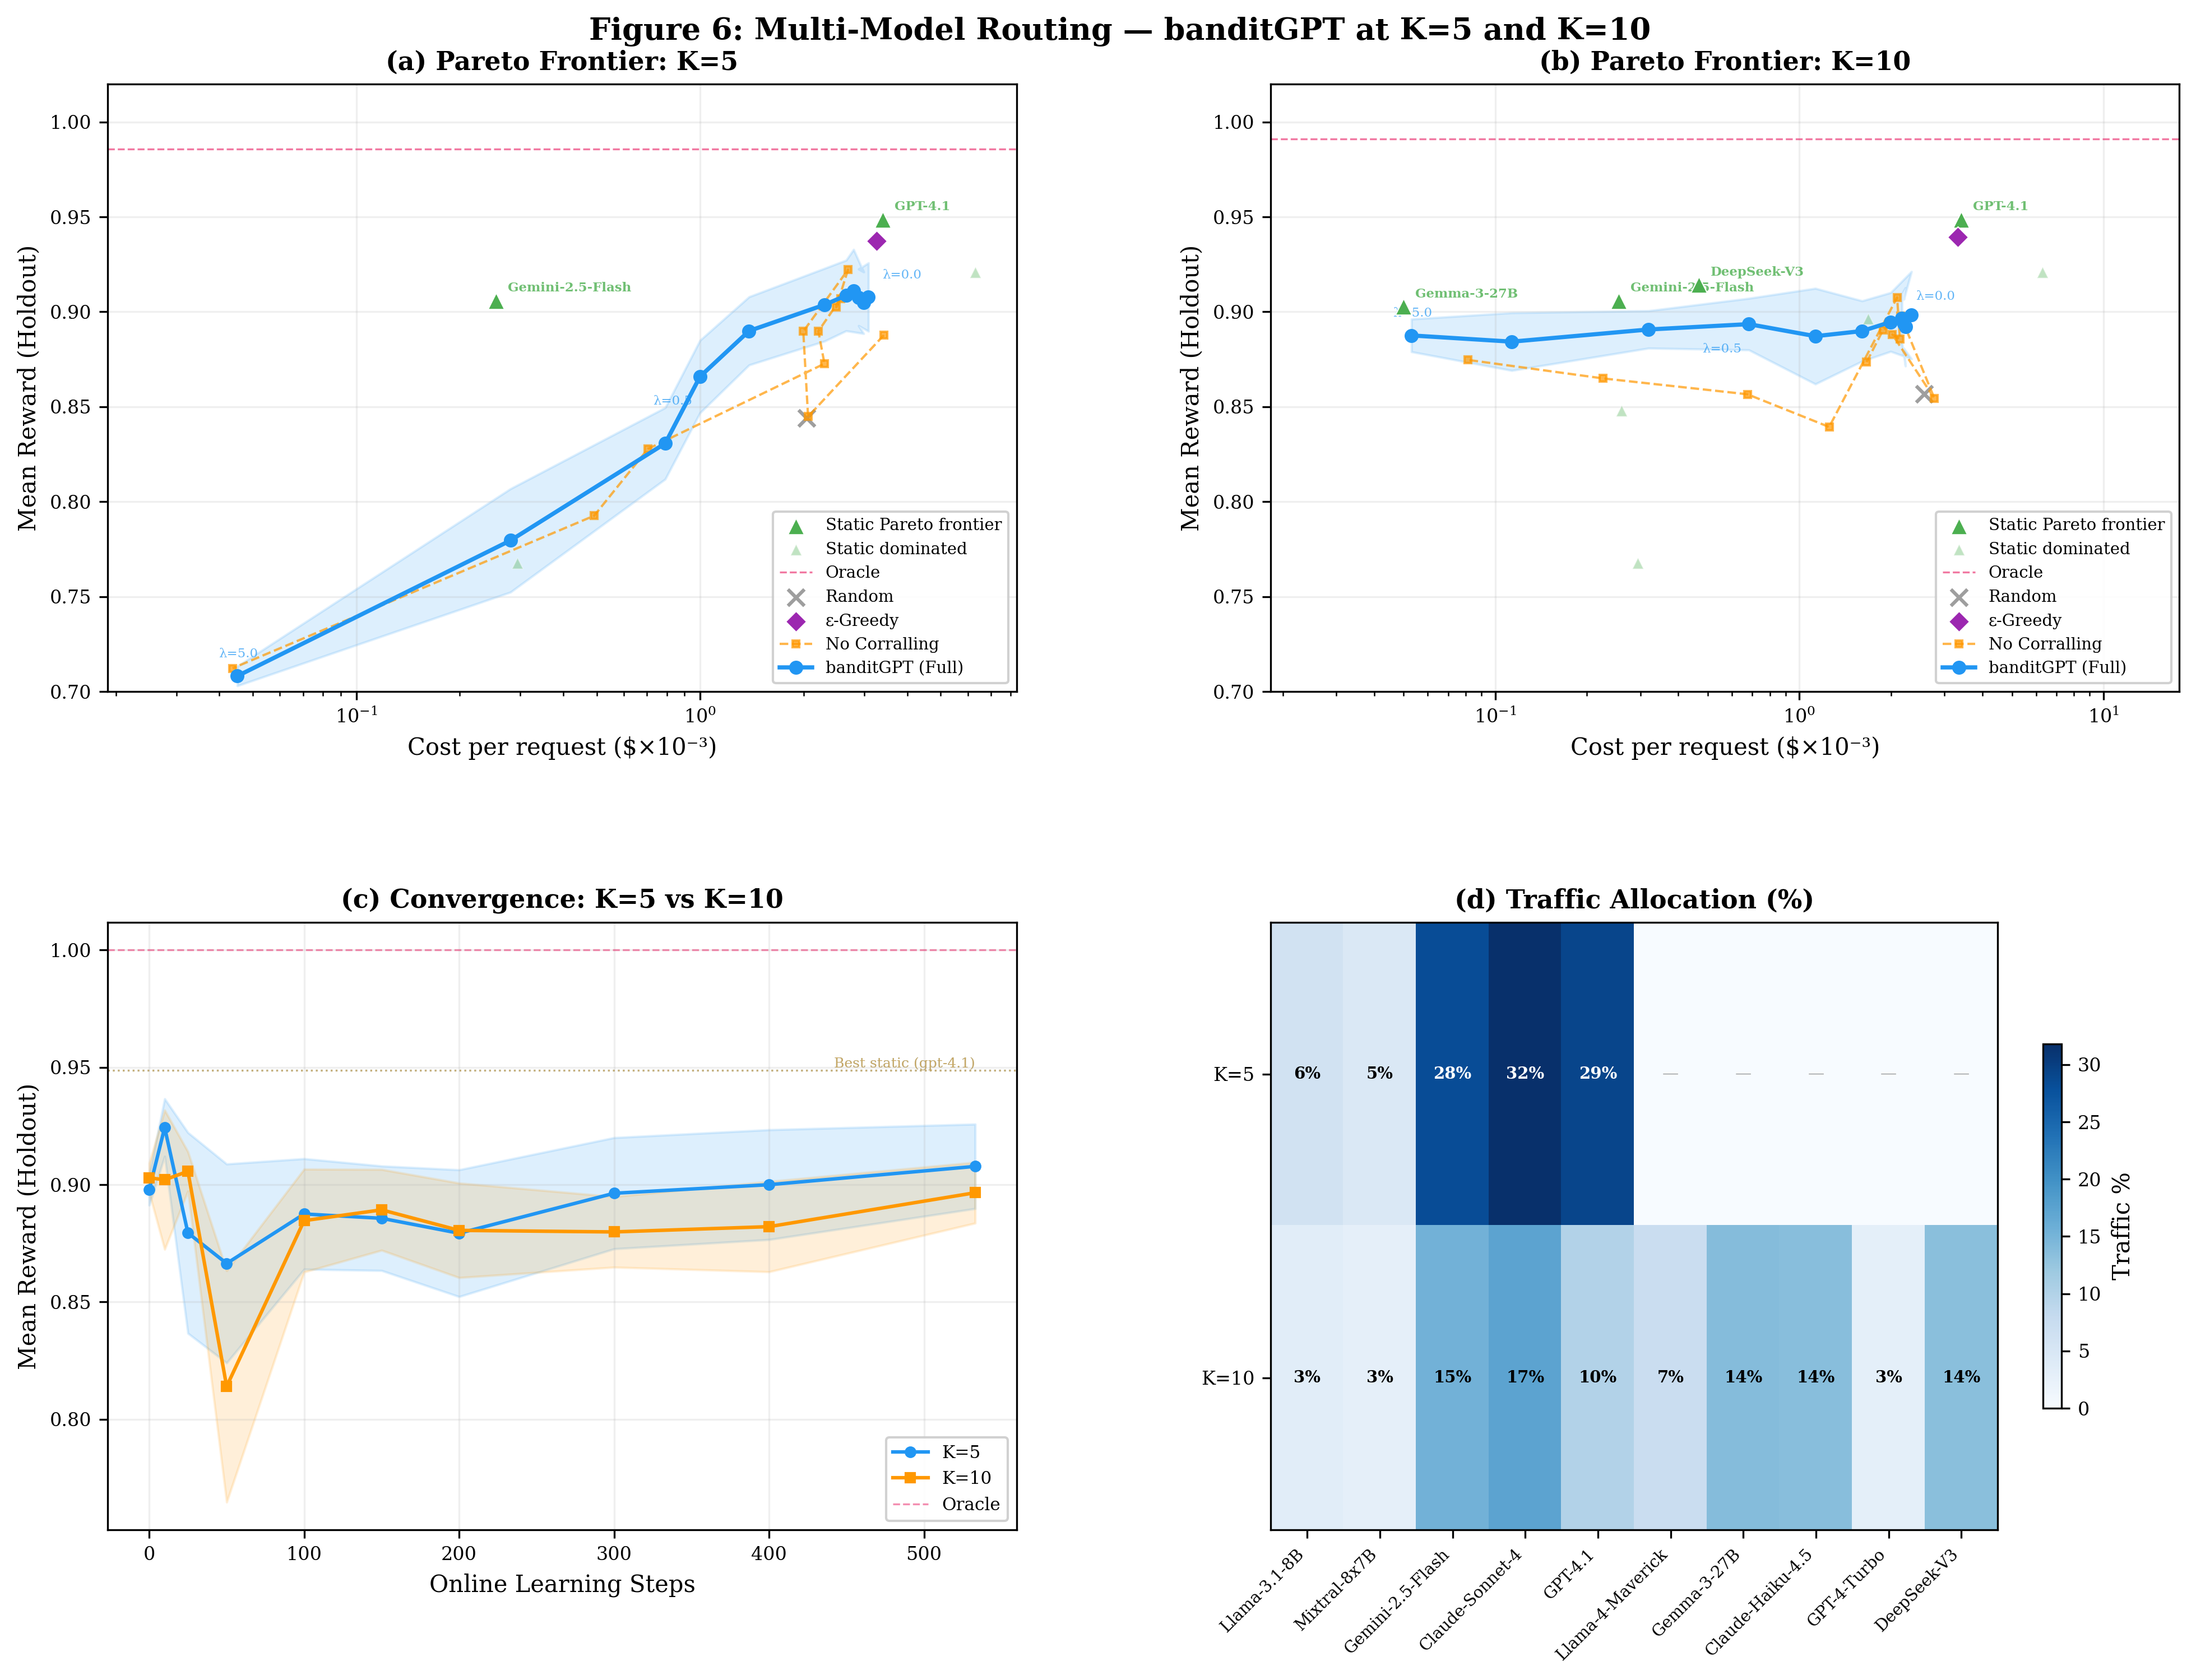
\includegraphics[width=0.95\textwidth]{../experiments/06_figure/results/figure6_multimodel_pareto.png}
\caption{\textbf{Multi-model routing at $K{=}5$ and $K{=}10$: cost--quality Pareto frontiers, convergence, and traffic allocation.} Reward is mean judge agreement across a 3--4 member LLM panel (continuous in $[0,1]$).
\textbf{(a,b)}~Pareto frontiers sweeping cost penalty $\lambda \in [0, 5]$ ($n{=}20$ seeds per point; log-scaled cost axis). Labelled green triangles mark Pareto-efficient static baselines; faded triangles show dominated models. The blue curve traces banditGPT's operating envelope. At peak quality ($\lambda{=}0.02$), banditGPT achieves 0.911 (K{=}5) and 0.898 (K{=}10). At $\lambda{=}5$ (cost-minimising), it routes nearly all traffic to the cheapest model while maintaining 0.708 (K{=}5) and 0.888 (K{=}10) quality. The orange dashed line (no Corralling) shows the ablated system without the meta-learner.
\textbf{(c)}~Convergence from warmup priors: both portfolios start at ${\sim}0.90$ reward (step~0, no online learning), demonstrating that the 43-model warmup priors provide effective cold-start quality across portfolio sizes. K{=}5 improves to 0.911 by step 533; K{=}10 remains stable at ${\sim}0.88{-}0.90$.
\textbf{(d)}~Traffic allocation on the holdout set ($\lambda{=}0$). At K{=}5, the router concentrates on three high-quality models (Claude-Sonnet: 32\%, GPT-4.1: 29\%, Gemini-Flash: 28\%) while using cheaper models sparingly (${\leq}6\%$). At K{=}10, traffic distributes across all models (3--17\% each), reflecting contextual per-prompt routing rather than static model selection.
Evaluation protocol: 533 online-learning prompts (three-way split, disjoint from prior training), frozen holdout of 750 prompts (identical to Section~\ref{sec:pareto}).}
\label{fig:multimodel_pareto}
\end{figure*}


\begin{figure*}[t]
\centering
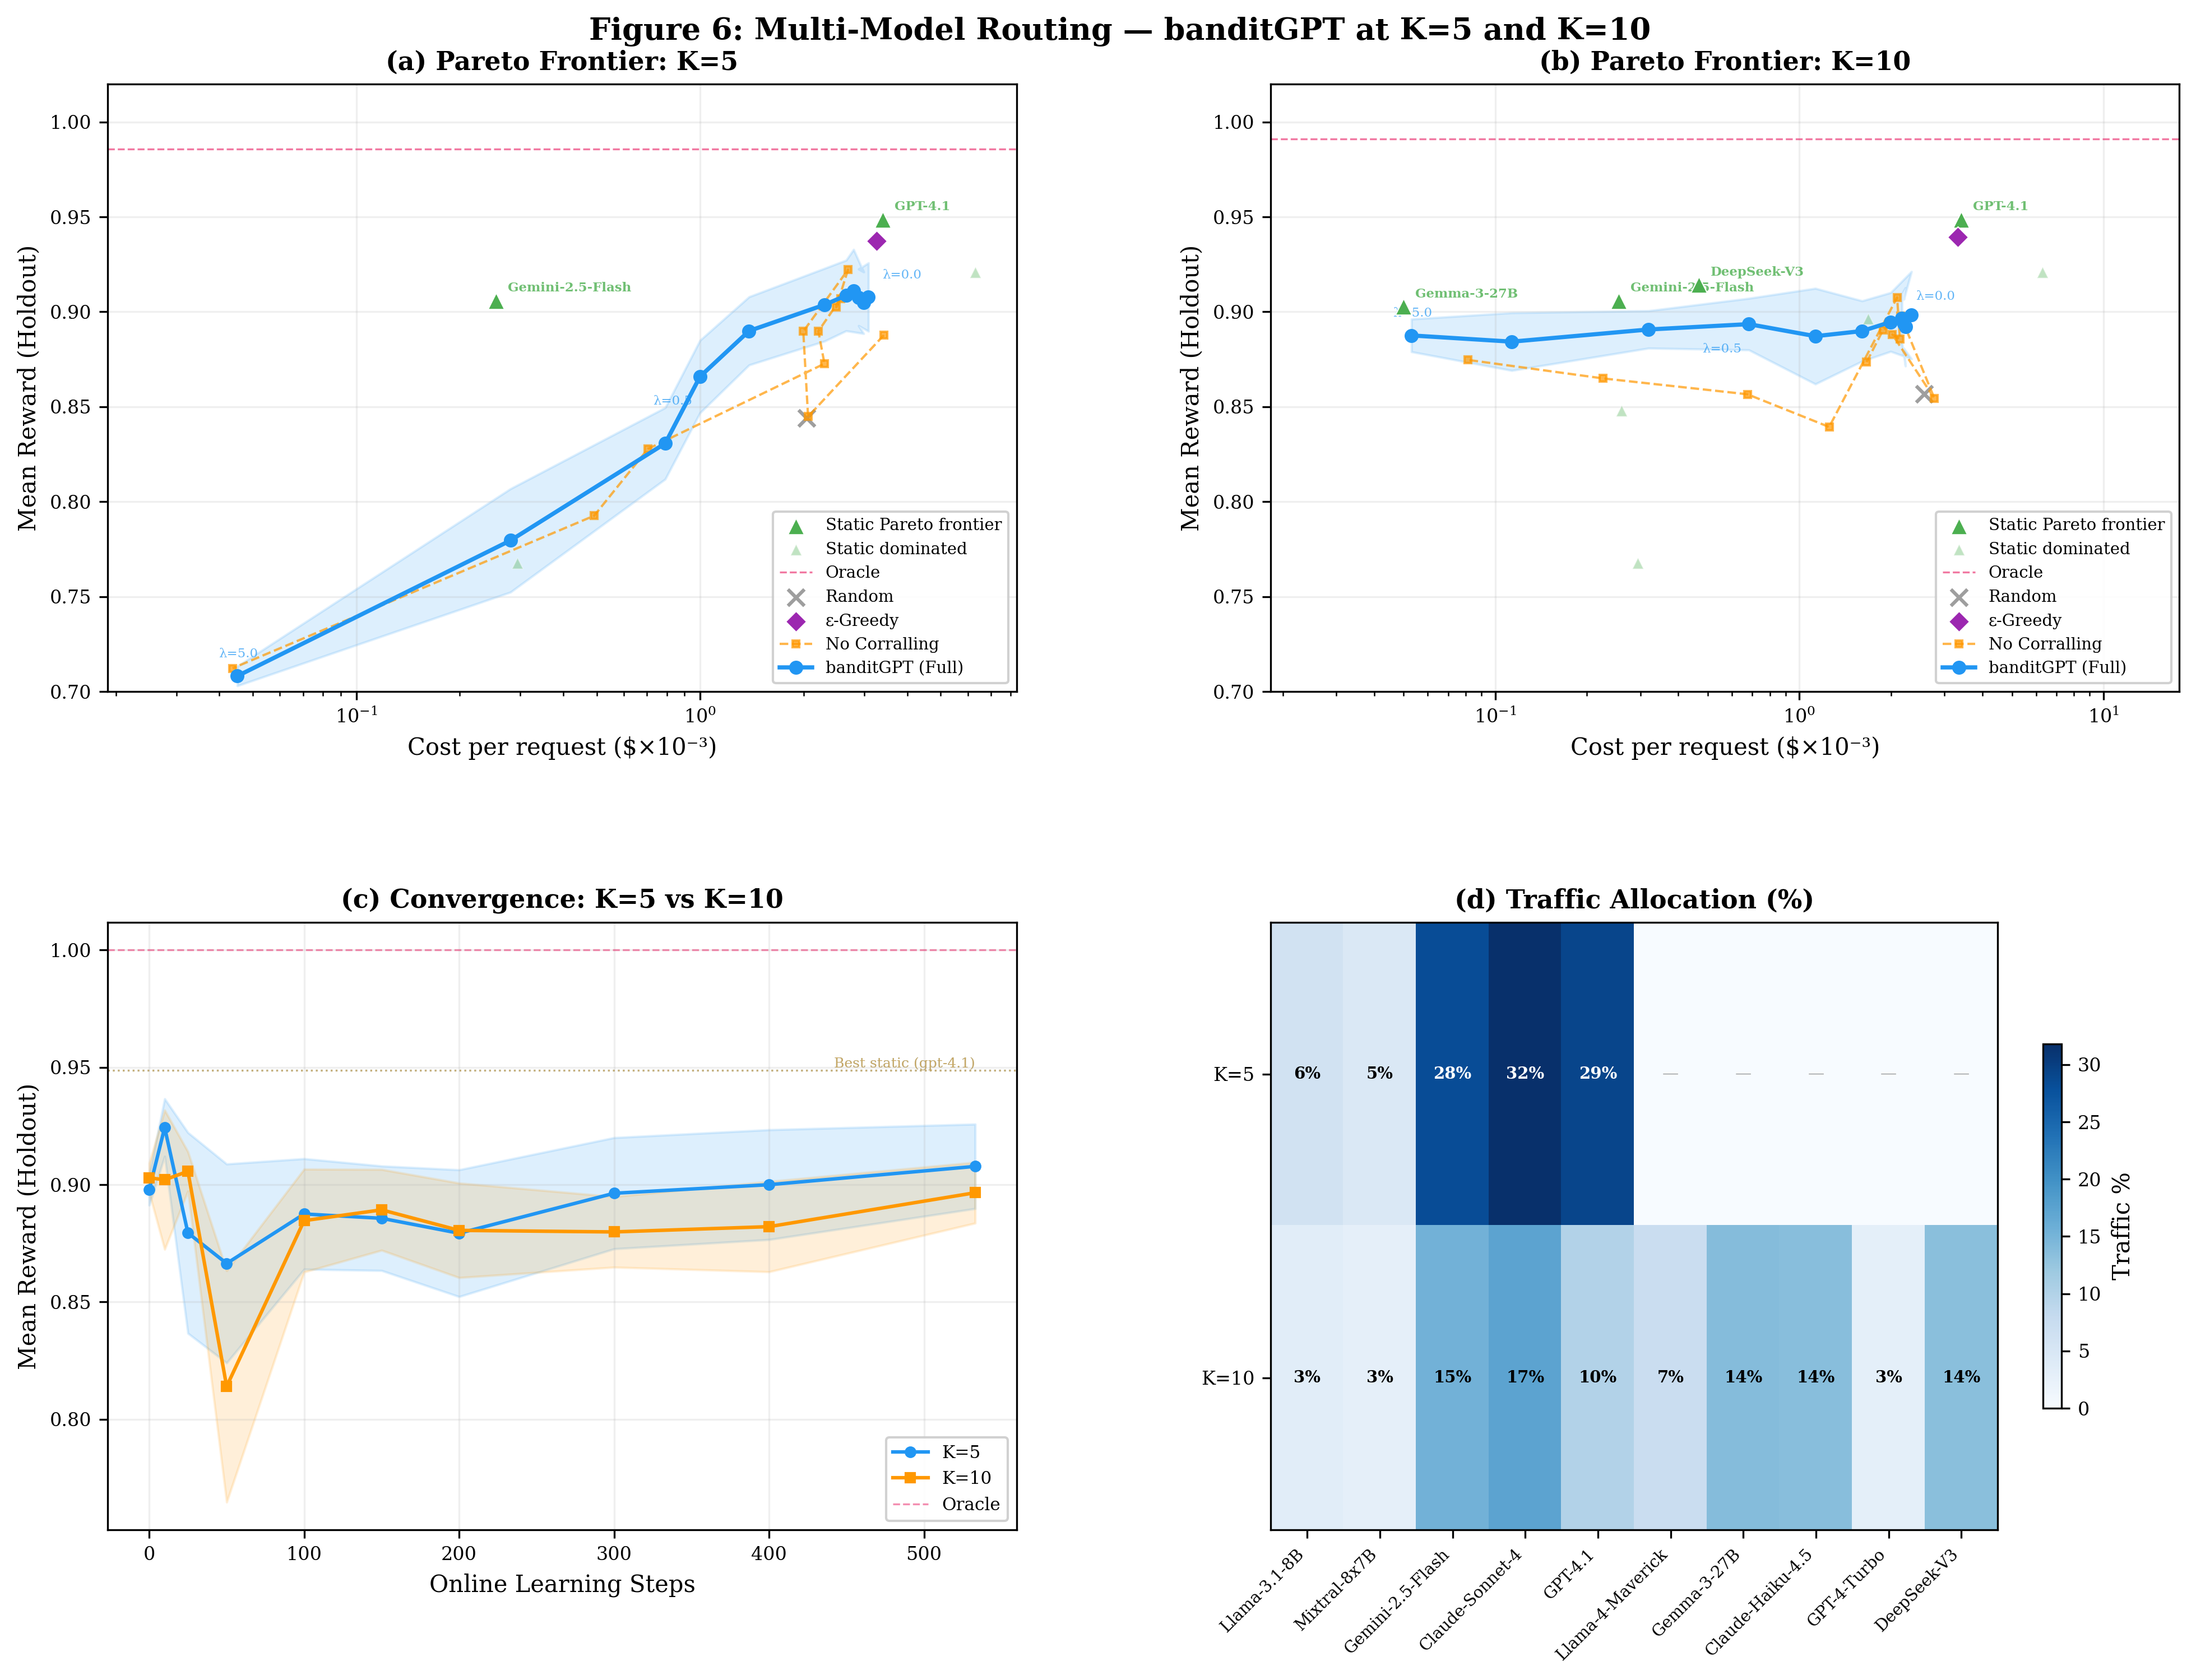
\includegraphics[width=0.95\textwidth]{../experiments/06_figure/results/figure6_multimodel_pareto.png}
\caption{\textbf{Multi-model routing at $K{=}5$ and $K{=}10$: cost--quality Pareto frontiers, convergence, and traffic allocation.} Reward is mean judge agreement across a 3--4 member LLM panel (continuous in $[0,1]$).
\textbf{(a,b)}~Pareto frontiers sweeping cost penalty $\lambda \in [0, 5]$ ($n{=}20$ seeds per point; log-scaled cost axis). Labelled green triangles mark Pareto-efficient static baselines; faded triangles show dominated models. The blue curve traces banditGPT's operating envelope. At peak quality ($\lambda{=}0.02$), banditGPT achieves 0.911 (K{=}5) and 0.898 (K{=}10). At $\lambda{=}5$ (cost-minimising), it routes nearly all traffic to the cheapest model while maintaining 0.708 (K{=}5) and 0.888 (K{=}10) quality. The orange dashed line (no Corralling) shows the ablated system without the meta-learner.
\textbf{(c)}~Convergence from warmup priors: both portfolios start at ${\sim}0.90$ reward (step~0, no online learning), demonstrating that the 43-model warmup priors provide effective cold-start quality across portfolio sizes. K{=}5 improves to 0.911 by step 533; K{=}10 remains stable at ${\sim}0.88{-}0.90$.
\textbf{(d)}~Traffic allocation on the holdout set ($\lambda{=}0$). At K{=}5, the router concentrates on three high-quality models (Claude-Sonnet: 32\%, GPT-4.1: 29\%, Gemini-Flash: 28\%) while using cheaper models sparingly (${\leq}6\%$). At K{=}10, traffic distributes across all models (3--17\% each), reflecting contextual per-prompt routing rather than static model selection.
Evaluation protocol: 533 online-learning prompts (three-way split, disjoint from prior training), frozen holdout of 750 prompts (identical to Section~\ref{sec:pareto}).}
\label{fig:multimodel_pareto}
\end{figure*}


\paragraph{Continuous cost--quality control.}
Table~\ref{tab:multimodel_summary} and Figure~\ref{fig:multimodel_pareto} summarize the findings. By sweeping a single scalar ($\lambda$), the router traces a smooth operating envelope. At $K{=}10$, quality degrades only 1\% ($0.898 \to 0.888$) across a $41\times$ cost range because the portfolio contains cheap, high-quality models (Gemma-3-27B, DeepSeek-V3) that the router leverages at higher $\lambda$ values.

\begin{table}[h]
\centering
\caption{Multi-model routing summary (mean judge agreement). Gap closure is relative to the weakest model. Mean $\pm$ std ($n{=}20$).}
\label{tab:multimodel_summary}
\small
\resizebox{\columnwidth}{!}{%
\begin{tabular}{@{}lcc@{}}
\toprule
\textbf{Metric} & \textbf{K=5} & \textbf{K=10} \\
\midrule
Oracle                     & 0.986              & 0.991 \\
Best Static (GPT-4.1)      & 0.949              & 0.949 \\
Random                     & 0.844 $\pm$ 0.008  & 0.857 $\pm$ 0.007 \\
\midrule
banditGPT Peak Quality     & 0.911 $\pm$ 0.022  & 0.898 $\pm$ 0.023 \\
Gap Closure                & 74.9\%              & 69.3\% \\
Warmup Cold-Start (step 0) & 0.898 $\pm$ 0.007  & 0.903 $\pm$ 0.006 \\
\midrule
Cost vs.\ Best Static at $\lambda{=}0$ & 9\% cheaper         & 36\% cheaper \\
Cost vs.\ Best Static at $\lambda{=}5$ & 98.7\% cheaper      & 98.4\% cheaper \\
\bottomrule
\end{tabular}%
}
\end{table}

\paragraph{Zero cold-start and distributed traffic.}
At step~0 (before online learning), banditGPT achieves holdout quality within 9\% of the Oracle. Online, traffic distributes across the portfolio based on prompt context. At $K{=}5$, three strong models share ${\sim}90\%$ of traffic; at $K{=}10$, no model exceeds 17\% (Figure~\ref{fig:multimodel_pareto}d). This provides immense operational resilience: a single-provider outage limits impact to a fraction of traffic, which the router autonomously redistributes.

\paragraph{Exploration-exploitation overhead.}
At peak $\lambda$, banditGPT's quality is slightly below the best static model (GPT-4.1). This reflects the bandit's structural exploration cost (testing sub-optimal models to verify calibration), which grows with $K$. However, this exploration enables a $91\%$ cost reduction at $\lambda{=}1.0$ relative to static GPT-4.1 with only a 6.1\% quality drop, a trade-off inaccessible to static baselines.

\paragraph{Static Pareto frontier and per-prompt value.}
The static Pareto frontier in Figure~\ref{fig:multimodel_pareto}(a,b) reveals which models are non-dominated when routing all traffic to a single endpoint. At $K{=}5$, only three of five models are Pareto-efficient (Llama-3.1-8B, Gemini-2.5-Flash, GPT-4.1); Mixtral-8x7B is dominated by Gemini-Flash (cheaper \emph{and} higher quality), and Claude-Sonnet-4 is dominated by GPT-4.1. Yet banditGPT routes 32\% of $K{=}5$ traffic to Claude-Sonnet-4 (Figure~\ref{fig:multimodel_pareto}d), indicating it provides unique value on specific prompt subsets despite being dominated in aggregate. This disconnect between aggregate dominance and per-prompt utility is precisely the Quality Inversion phenomenon that contextual routing exploits: a model that is strictly inferior on average can still be the best choice for a measurable fraction of prompts.


\subsection{Multi-Model Cost--Quality Trade-off ($K{=}5, 10$)}
\label{sec:multimodel}

We construct two multi-provider portfolios ($K{=}5$ and $K{=}10$) spanning six providers (Meta, Mistral, Google, Anthropic, OpenAI, DeepSeek) with a $600\times$ cost spread. Both incorporate Mixtral-8x7B to link to the $K{=}2$ evaluation, and $K{=}10$ exercises Hybrid LinUCB's within-family parameter sharing. Warmup priors are generated using a three-way split from 43-model evaluation data (355 prior training prompts, 533 online learning, 750 holdout).

% Figure 6: Multi-Model Pareto Frontier — K=5 and K=10
% Include from the main paper via % Figure 6: Multi-Model Pareto Frontier — K=5 and K=10
% Include from the main paper via % Figure 6: Multi-Model Pareto Frontier — K=5 and K=10
% Include from the main paper via \input{../experiments/06_figure/figure_6_caption}

\begin{figure*}[t]
\centering
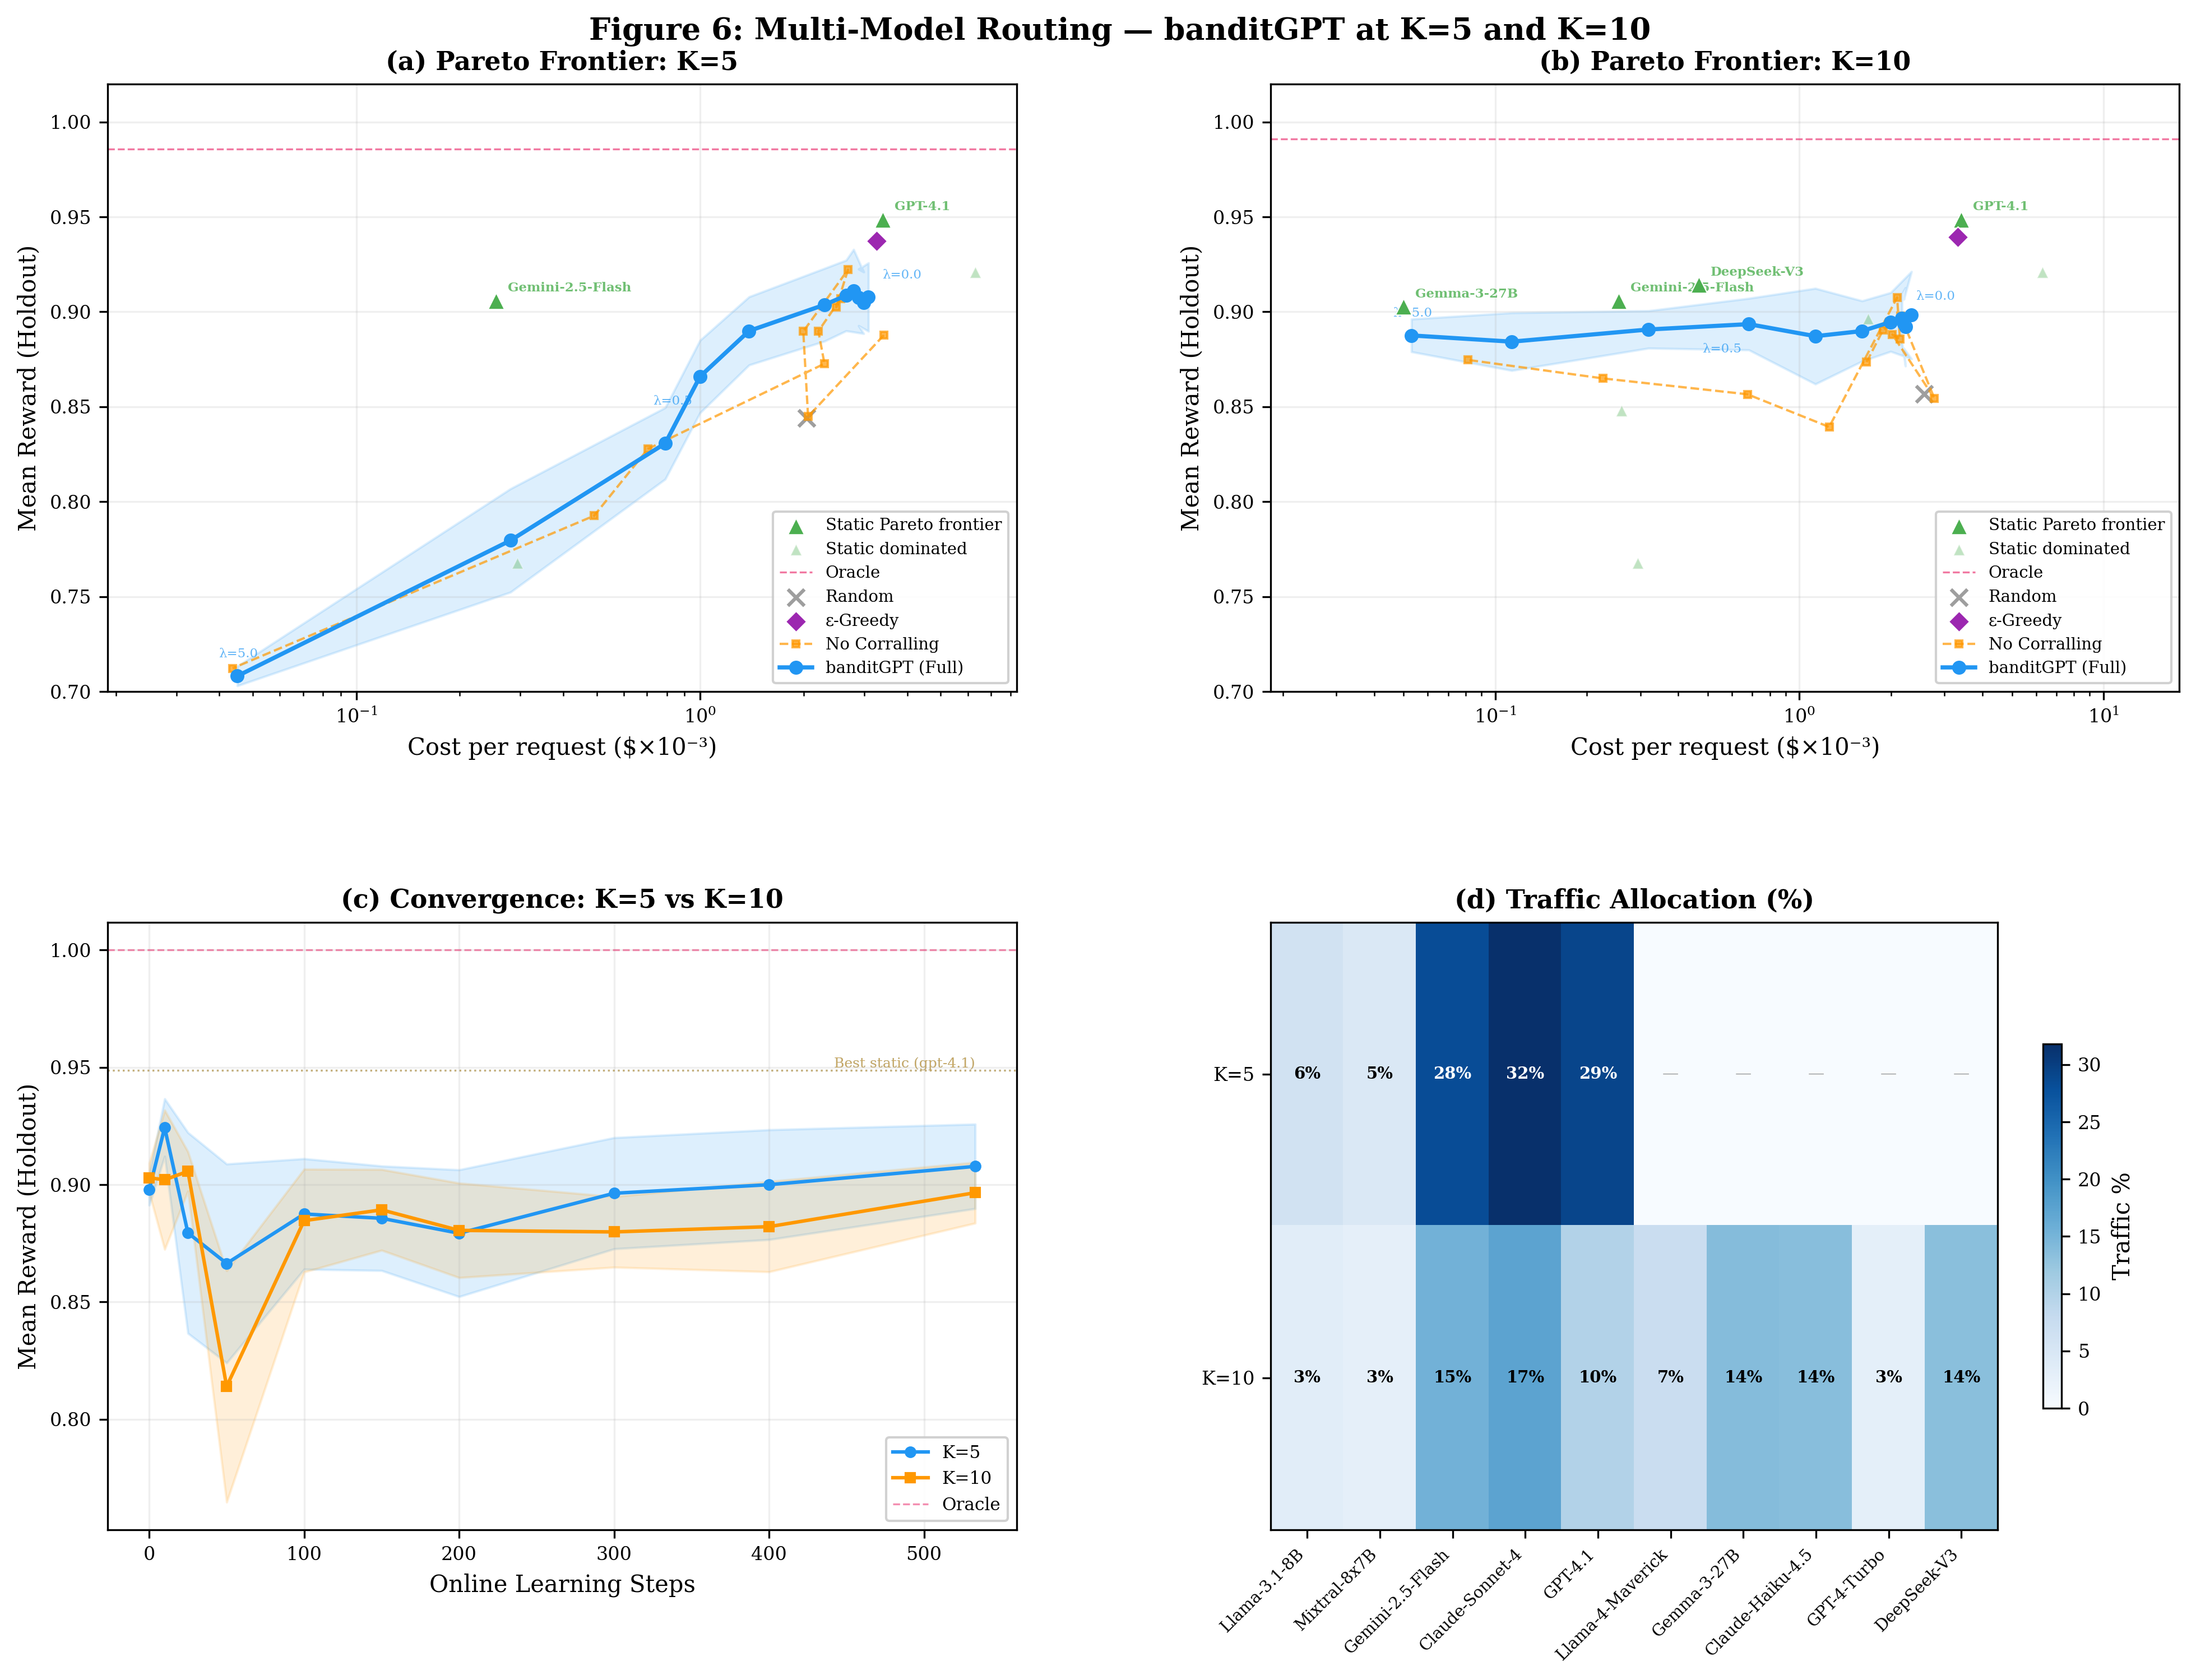
\includegraphics[width=0.95\textwidth]{../experiments/06_figure/results/figure6_multimodel_pareto.png}
\caption{\textbf{Multi-model routing at $K{=}5$ and $K{=}10$: cost--quality Pareto frontiers, convergence, and traffic allocation.} Reward is mean judge agreement across a 3--4 member LLM panel (continuous in $[0,1]$).
\textbf{(a,b)}~Pareto frontiers sweeping cost penalty $\lambda \in [0, 5]$ ($n{=}20$ seeds per point; log-scaled cost axis). Labelled green triangles mark Pareto-efficient static baselines; faded triangles show dominated models. The blue curve traces banditGPT's operating envelope. At peak quality ($\lambda{=}0.02$), banditGPT achieves 0.911 (K{=}5) and 0.898 (K{=}10). At $\lambda{=}5$ (cost-minimising), it routes nearly all traffic to the cheapest model while maintaining 0.708 (K{=}5) and 0.888 (K{=}10) quality. The orange dashed line (no Corralling) shows the ablated system without the meta-learner.
\textbf{(c)}~Convergence from warmup priors: both portfolios start at ${\sim}0.90$ reward (step~0, no online learning), demonstrating that the 43-model warmup priors provide effective cold-start quality across portfolio sizes. K{=}5 improves to 0.911 by step 533; K{=}10 remains stable at ${\sim}0.88{-}0.90$.
\textbf{(d)}~Traffic allocation on the holdout set ($\lambda{=}0$). At K{=}5, the router concentrates on three high-quality models (Claude-Sonnet: 32\%, GPT-4.1: 29\%, Gemini-Flash: 28\%) while using cheaper models sparingly (${\leq}6\%$). At K{=}10, traffic distributes across all models (3--17\% each), reflecting contextual per-prompt routing rather than static model selection.
Evaluation protocol: 533 online-learning prompts (three-way split, disjoint from prior training), frozen holdout of 750 prompts (identical to Section~\ref{sec:pareto}).}
\label{fig:multimodel_pareto}
\end{figure*}


\begin{figure*}[t]
\centering
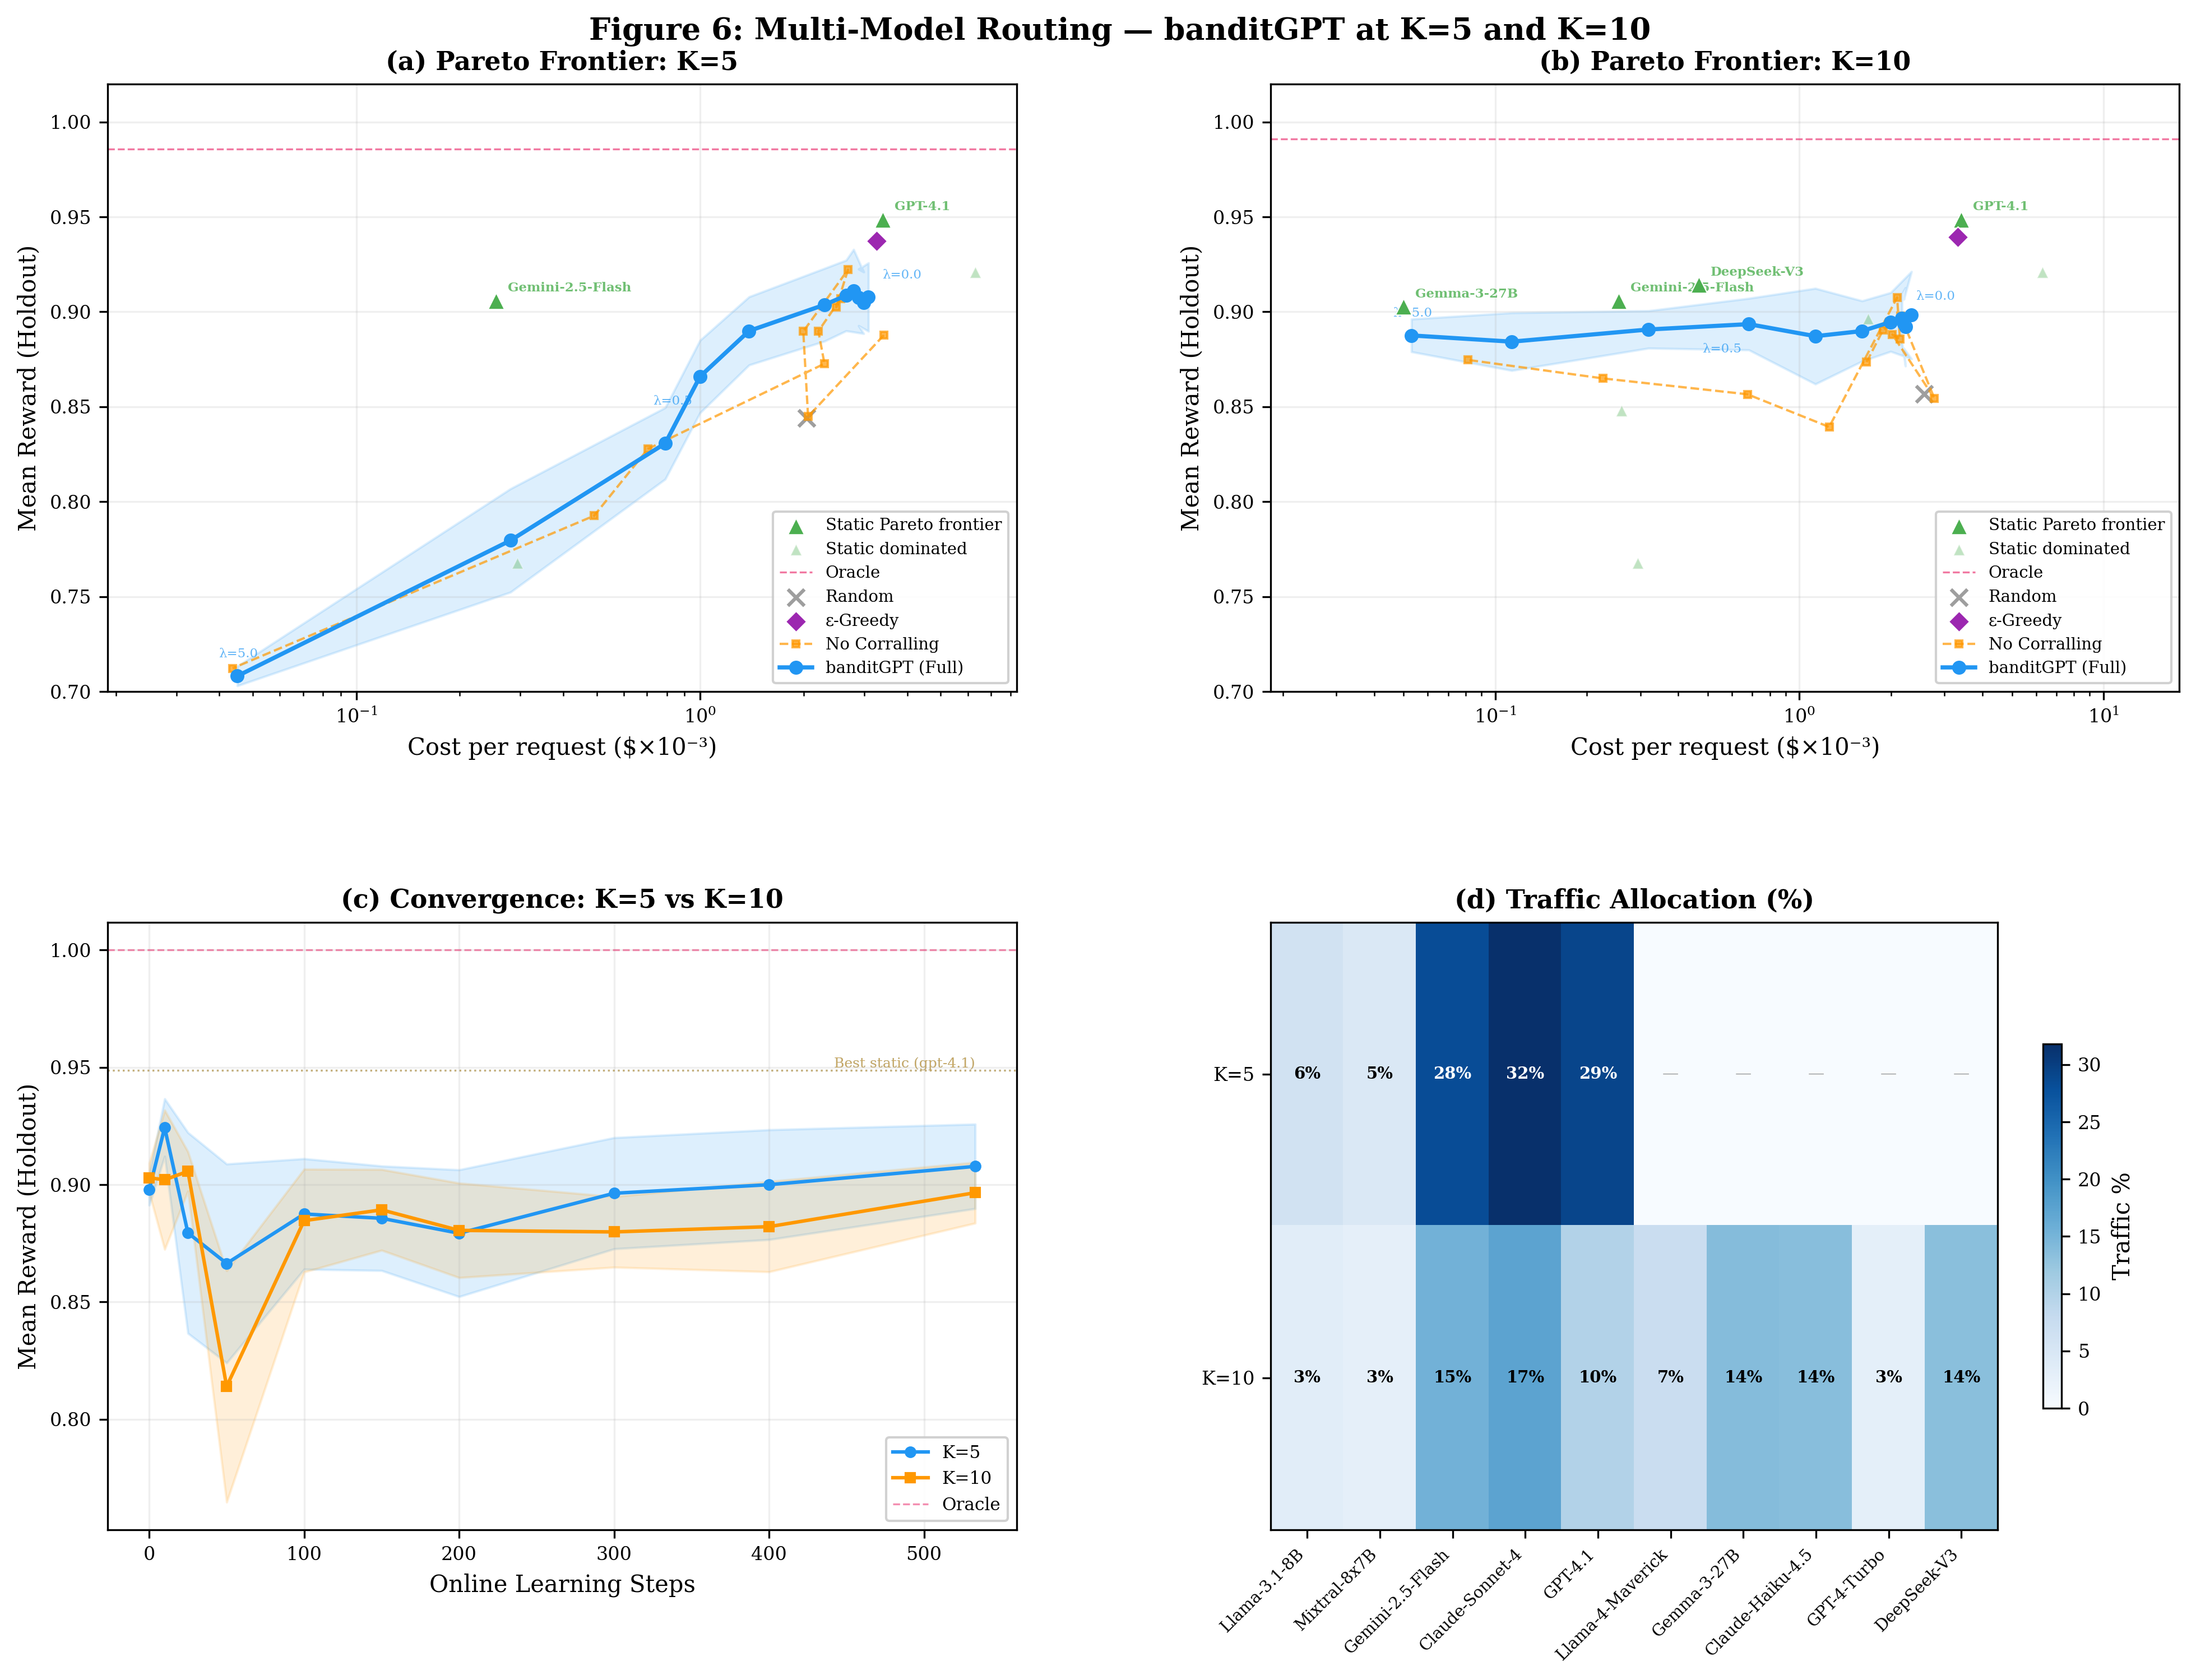
\includegraphics[width=0.95\textwidth]{../experiments/06_figure/results/figure6_multimodel_pareto.png}
\caption{\textbf{Multi-model routing at $K{=}5$ and $K{=}10$: cost--quality Pareto frontiers, convergence, and traffic allocation.} Reward is mean judge agreement across a 3--4 member LLM panel (continuous in $[0,1]$).
\textbf{(a,b)}~Pareto frontiers sweeping cost penalty $\lambda \in [0, 5]$ ($n{=}20$ seeds per point; log-scaled cost axis). Labelled green triangles mark Pareto-efficient static baselines; faded triangles show dominated models. The blue curve traces banditGPT's operating envelope. At peak quality ($\lambda{=}0.02$), banditGPT achieves 0.911 (K{=}5) and 0.898 (K{=}10). At $\lambda{=}5$ (cost-minimising), it routes nearly all traffic to the cheapest model while maintaining 0.708 (K{=}5) and 0.888 (K{=}10) quality. The orange dashed line (no Corralling) shows the ablated system without the meta-learner.
\textbf{(c)}~Convergence from warmup priors: both portfolios start at ${\sim}0.90$ reward (step~0, no online learning), demonstrating that the 43-model warmup priors provide effective cold-start quality across portfolio sizes. K{=}5 improves to 0.911 by step 533; K{=}10 remains stable at ${\sim}0.88{-}0.90$.
\textbf{(d)}~Traffic allocation on the holdout set ($\lambda{=}0$). At K{=}5, the router concentrates on three high-quality models (Claude-Sonnet: 32\%, GPT-4.1: 29\%, Gemini-Flash: 28\%) while using cheaper models sparingly (${\leq}6\%$). At K{=}10, traffic distributes across all models (3--17\% each), reflecting contextual per-prompt routing rather than static model selection.
Evaluation protocol: 533 online-learning prompts (three-way split, disjoint from prior training), frozen holdout of 750 prompts (identical to Section~\ref{sec:pareto}).}
\label{fig:multimodel_pareto}
\end{figure*}


\begin{figure*}[t]
\centering
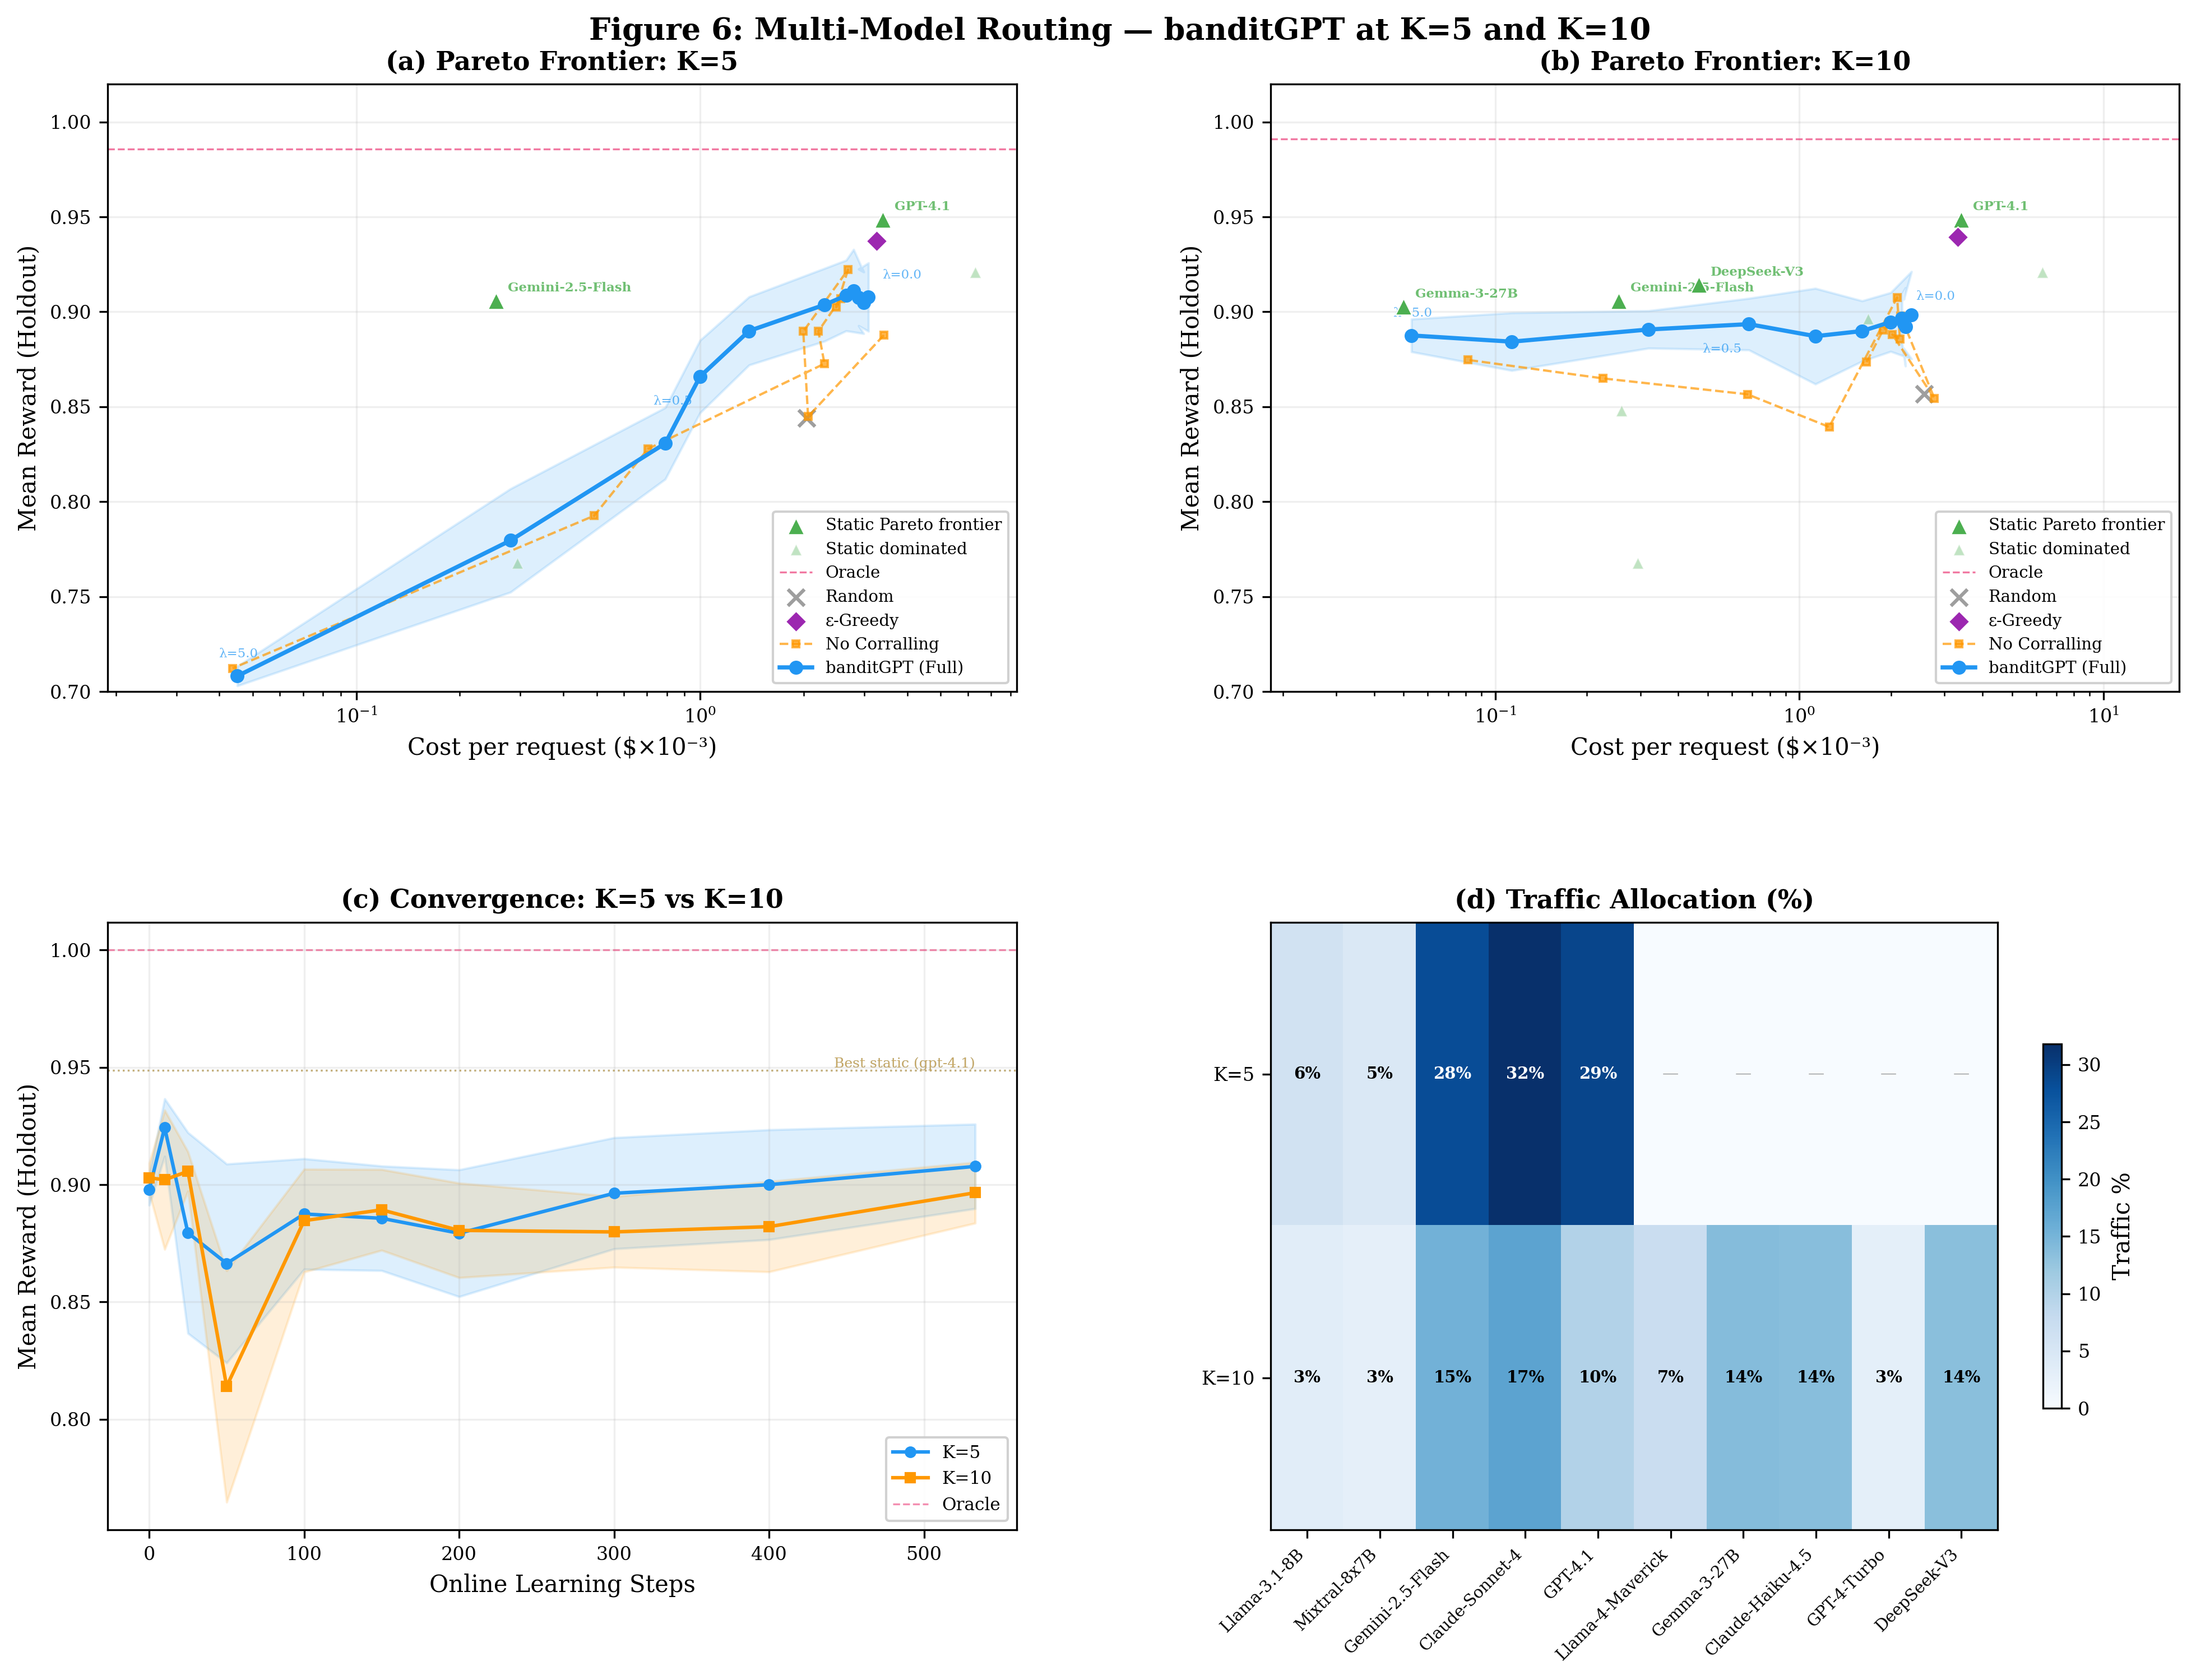
\includegraphics[width=0.95\textwidth]{../experiments/06_figure/results/figure6_multimodel_pareto.png}
\caption{\textbf{Multi-model routing at $K{=}5$ and $K{=}10$: cost--quality Pareto frontiers, convergence, and traffic allocation.} Reward is mean judge agreement across a 3--4 member LLM panel (continuous in $[0,1]$).
\textbf{(a,b)}~Pareto frontiers sweeping cost penalty $\lambda \in [0, 5]$ ($n{=}20$ seeds per point; log-scaled cost axis). Labelled green triangles mark Pareto-efficient static baselines; faded triangles show dominated models. The blue curve traces banditGPT's operating envelope. At peak quality ($\lambda{=}0.02$), banditGPT achieves 0.911 (K{=}5) and 0.898 (K{=}10). At $\lambda{=}5$ (cost-minimising), it routes nearly all traffic to the cheapest model while maintaining 0.708 (K{=}5) and 0.888 (K{=}10) quality. The orange dashed line (no Corralling) shows the ablated system without the meta-learner.
\textbf{(c)}~Convergence from warmup priors: both portfolios start at ${\sim}0.90$ reward (step~0, no online learning), demonstrating that the 43-model warmup priors provide effective cold-start quality across portfolio sizes. K{=}5 improves to 0.911 by step 533; K{=}10 remains stable at ${\sim}0.88{-}0.90$.
\textbf{(d)}~Traffic allocation on the holdout set ($\lambda{=}0$). At K{=}5, the router concentrates on three high-quality models (Claude-Sonnet: 32\%, GPT-4.1: 29\%, Gemini-Flash: 28\%) while using cheaper models sparingly (${\leq}6\%$). At K{=}10, traffic distributes across all models (3--17\% each), reflecting contextual per-prompt routing rather than static model selection.
Evaluation protocol: 533 online-learning prompts (three-way split, disjoint from prior training), frozen holdout of 750 prompts (identical to Section~\ref{sec:pareto}).}
\label{fig:multimodel_pareto}
\end{figure*}


\paragraph{Continuous cost--quality control.}
Table~\ref{tab:multimodel_summary} and Figure~\ref{fig:multimodel_pareto} summarize the findings. By sweeping a single scalar ($\lambda$), the router traces a smooth operating envelope. At $K{=}10$, quality degrades only 1\% ($0.898 \to 0.888$) across a $41\times$ cost range because the portfolio contains cheap, high-quality models (Gemma-3-27B, DeepSeek-V3) that the router leverages at higher $\lambda$ values.

\begin{table}[h]
\centering
\caption{Multi-model routing summary (mean judge agreement). Gap closure is relative to the weakest model. Mean $\pm$ std ($n{=}20$).}
\label{tab:multimodel_summary}
\small
\resizebox{\columnwidth}{!}{%
\begin{tabular}{@{}lcc@{}}
\toprule
\textbf{Metric} & \textbf{K=5} & \textbf{K=10} \\
\midrule
Oracle                     & 0.986              & 0.991 \\
Best Static (GPT-4.1)      & 0.949              & 0.949 \\
Random                     & 0.844 $\pm$ 0.008  & 0.857 $\pm$ 0.007 \\
\midrule
banditGPT Peak Quality     & 0.911 $\pm$ 0.022  & 0.898 $\pm$ 0.023 \\
Gap Closure                & 74.9\%              & 69.3\% \\
Warmup Cold-Start (step 0) & 0.898 $\pm$ 0.007  & 0.903 $\pm$ 0.006 \\
\midrule
Cost vs.\ Best Static at $\lambda{=}0$ & 9\% cheaper         & 36\% cheaper \\
Cost vs.\ Best Static at $\lambda{=}5$ & 98.7\% cheaper      & 98.4\% cheaper \\
\bottomrule
\end{tabular}%
}
\end{table}

\paragraph{Zero cold-start and distributed traffic.}
At step~0 (before online learning), banditGPT achieves holdout quality within 9\% of the Oracle. Online, traffic distributes across the portfolio based on prompt context. At $K{=}5$, three strong models share ${\sim}90\%$ of traffic; at $K{=}10$, no model exceeds 17\% (Figure~\ref{fig:multimodel_pareto}d). This provides immense operational resilience: a single-provider outage limits impact to a fraction of traffic, which the router autonomously redistributes.

\paragraph{Exploration-exploitation overhead.}
At peak $\lambda$, banditGPT's quality is slightly below the best static model (GPT-4.1). This reflects the bandit's structural exploration cost (testing sub-optimal models to verify calibration), which grows with $K$. However, this exploration enables a $91\%$ cost reduction at $\lambda{=}1.0$ relative to static GPT-4.1 with only a 6.1\% quality drop, a trade-off inaccessible to static baselines.

\paragraph{Static Pareto frontier and per-prompt value.}
The static Pareto frontier in Figure~\ref{fig:multimodel_pareto}(a,b) reveals which models are non-dominated when routing all traffic to a single endpoint. At $K{=}5$, only three of five models are Pareto-efficient (Llama-3.1-8B, Gemini-2.5-Flash, GPT-4.1); Mixtral-8x7B is dominated by Gemini-Flash (cheaper \emph{and} higher quality), and Claude-Sonnet-4 is dominated by GPT-4.1. Yet banditGPT routes 32\% of $K{=}5$ traffic to Claude-Sonnet-4 (Figure~\ref{fig:multimodel_pareto}d), indicating it provides unique value on specific prompt subsets despite being dominated in aggregate. This disconnect between aggregate dominance and per-prompt utility is precisely the Quality Inversion phenomenon that contextual routing exploits: a model that is strictly inferior on average can still be the best choice for a measurable fraction of prompts.
